\documentclass[12pt]{article}

\usepackage[a4paper, left=1.2in, right=1.2in]{geometry}
\usepackage{setspace}
\usepackage[utf8]{inputenc}
\usepackage[italian]{babel}
\usepackage[OT1]{fontenc}
\usepackage{graphicx}
\usepackage{subcaption}
\usepackage{float}
\usepackage{fancyhdr}
\usepackage{xcolor}
\usepackage{mathtools}
\usepackage{amsmath}
\usepackage{amssymb}
\usepackage{tikz}
\usepackage{imakeidx}
\usepackage{textcomp}
\usepackage{pifont}
\usepackage{polynom}
\usepackage{algorithm}
\usepackage{algpseudocode}
\usepackage{mathtools}
\usepackage[colorlinks=true,linkcolor=black,anchorcolor=black,citecolor=black,filecolor=black,menucolor=black,runcolor=black,urlcolor=black]{hyperref}
\usepackage{cancel}
\usepackage{pgfplots}
\usepackage{caption}
\usepackage{tabularx}
\usepackage{comment}
\usepackage{float}
\usepackage{bm}
\usepackage{multirow}

\onehalfspacing

\begin{document}
\bibliographystyle{plain}
    \pagestyle{fancy}
    \everymath{\displaystyle}
    \sffamily
\section{Sostenibilità e AI}
Con il termine sostenibilità intendiamo \textbf{la capacità di soddisfare bisogni attuali senza compromettere il futuro}.
La sostenibilità,dunque,riguarda la gestione responsabile delle risorse naturali, la tutela dell'ambiente, lo sviluppo economico e la giustizia sociale. L'Agenda 2030 per lo sviluppo sostenibile, rappresenta un impegno globale per la sostenibilità, con 17 obiettivi.
Tra tutti questi obiettivi diversi fanno riferimento alla sostenibilità ambientale, cioè il     \textbf{mantenimento del capitale naturale}, ovvero non consumare più risorse di quelle che la natura è in grado di rigenerare. Spostandoci in campo Intelligenza Artificiali, in relazione all'impatto ambientale possiamo distinguere due tipologie:
\begin{itemize}
    \item \textcolor{green}{Green AI}: si riferisce allo sviluppo sostenibile
    \item \textcolor{red}{Dirty AI}: si riferisce allo sviluppo non sostenibile
\end{itemize}

\section{RecSys}
Un sistema di raccomandazione è un sistema software progettato per suggerire all’utente elementi di interesse, come ad esempio prodotti, servizi, informazioni o contenuti multimediali, in base alle preferenze e ai comportamenti passati dell’utente. Si basano su tecniche di Intelligenza Artificiale e Machine Learning. I RecSys possono essere di diversi tipi:
\begin{itemize}
    \item \textbf{Content-based}: si basano sul contenuto degli oggetti raccomandati
    \item \textbf{Collaborative filtering}: si basano sulle preferenze degli utenti
    \item \textbf{Knowledge-aware}: si basano su conoscenze esterne
    \item \textbf{Hybrid}: combinano le tecniche precedenti
\end{itemize}

\section{Research Question}

• RQ1: Qual è il trade-off tra emissioni e performance dei modelli di raccomandazione a stato dell’arte1?\\
• RQ2: E’ possibile usare un criterio di early-stopping basato sulle emissioni per migliorare il trade-off tra emissioni e performance dei modelli di raccomandazione a stato dell’arte?\\
• RQ3: Quali parametri possono essere utilizzati in questi criteri per migliorare il trade-off?
\section{Riassunto lavoro}
\begin{figure}[H]
    \centering
    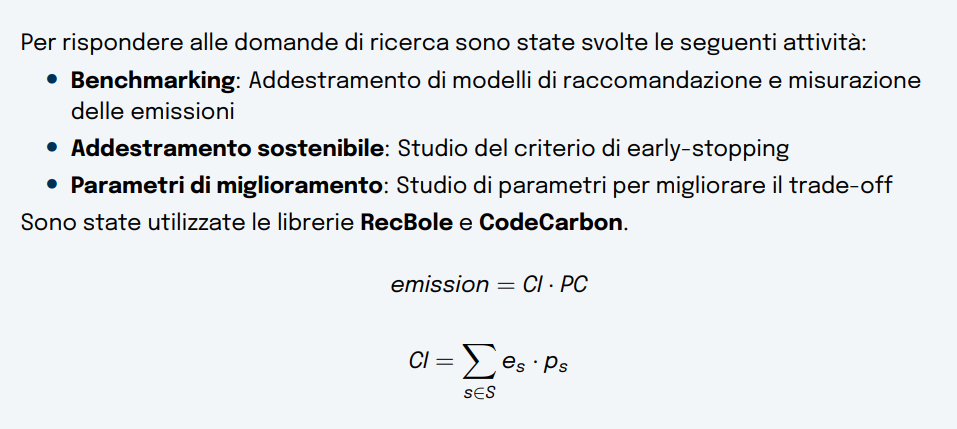
\includegraphics[width=0.8\textwidth]{image.png}
    \caption{Riassunto del lavoro}
    \label{fig:riassunto}
\end{figure}
In particolare per PC intendiamo la Power Consumption, mentre per CI intendiamo la Carbon Intensity, la quale è data dalla sommatoria di energia prodotta da una certa fonte moltiplicata per il suo fattore di emissione.\\
\end{document}